\documentclass{report}
\usepackage{ctex}
\usepackage{graphicx}
\usepackage{amsmath}
\title{半导体温度计的设计和制作}
\author{王启骅 PB20020580}
\begin{document}
	\maketitle
	\section{实验目的}
	用半导体热敏电阻作为温度传感器,设计制作一个半导体温度计,温度测量范围:20~70 ℃。设计制作相应的测温电路,实现测量要求。
	\section{实验原理}
	半导体电阻值随温度变化关系:\\
		$ R_T=R_{\infty}e^{\frac{B}{T}} $\\

	电阻随温度升高而急剧降低,通过测量其阻值来确定温度。\\
	热敏电阻伏安曲线的起始部分接近线性,电流的影响可以忽略不计,热敏电阻的阻值主要与外界温度有关,在温度计设计
	制作过程中要使热敏电阻工作在其小电流的线性区。\\
	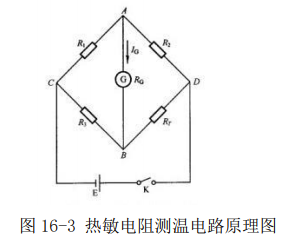
\includegraphics{1}\\
		在温度下限$ T_1 $时,微安计$ I_g=0 $此时热敏电阻值为$  R_{T_1} $,电桥处于平衡状态,满足平衡条件$ \frac{R_1}{R_2}=\frac{R_3}{R_{T_1}} $。取 R1=R2,则 R3=RT1。由此确定了 R3的电阻值即为热敏电阻处在测温量程的下限温度时的电阻值 RT1。
当温度增加时,热敏电阻的电阻值就会减小,电桥失去平衡,通过电路分析可以根据微安计的读数 IG的大小计算出 RT,从而得到$ I_G $与温度的关系。当达到上限温度$ T_2 $时,微安计满偏,可得$ V_{CD}=I_T(R_3+R) $\\
	由基尔霍夫方程:$ I_G=\dfrac{\dfrac{R_2}{R_1+R_2}-\dfrac{R_{T2}}{R_3+R_{T2}}}{R_G+\dfrac{R_1R_2}{R_1+R_2}+\dfrac{R_3R_{T2}}{R_3+R_{T2}}} $\\
	带入$ R_1=R_2,R_{T1}=R_3 $得:\\$ R_1=\frac{2V_{CD}}{I_G}(1/2-\dfrac{R_{T2}}{R_{T1}+R{T2}})-2(R_G+\dfrac{R_{T1}R_{T2}}{R_{T1}+R_{T2}}) $\\
	选取$ V_{CD}=1V $,保证热敏电阻工作于其伏安特性曲线的线性部分

	
	\section{实验仪器}
	实验仪器:烙铁、万用表、恒温水浴箱 2 个。
	电路元件:热敏电阻(温度特性给定)、微安计(内阻 Rg 已知)、可变电阻
	箱、电位器 5 个、1.5V 电池、多档开关、待焊接的电路板、导线若干。
	\section{实验数据}
	\begin{flushleft}
		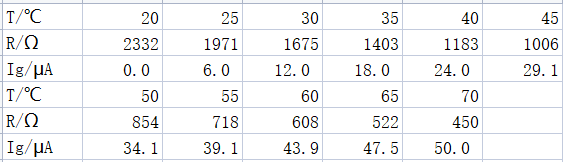
\includegraphics{2}	\\ 
		表1:半导体温度计标定原始数据表\\
		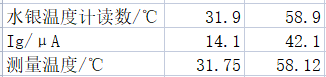
\includegraphics{3}	\\ 
		表2:温度计测试数据表
	\end{flushleft}

	\section{数据处理与误差分析}
半导体温度计标定:\\
	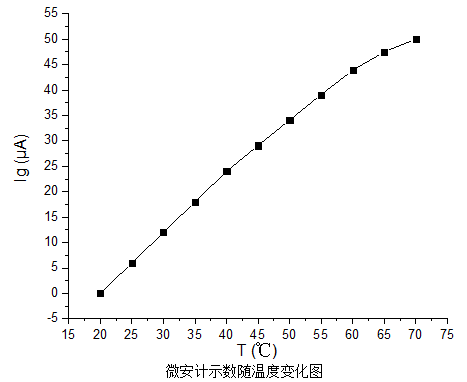
\includegraphics{4}

	温度计测试:\\
	$ \frac{\Delta T_1}{T_1}=\dfrac{31.9-31.75}{31.9}=0.5\% $\qquad
	$ \frac{\Delta T_2}{T_2}=\dfrac{58.9-58.12}{58.9}=1.3\% $
	
	
	\section{实验讨论}
	焊接好电路后要及时检查是否虚焊,以免实验时带来不便。调节好$ R_1,R_2,R_3,,R_4,R $后,应注意不要碰到调节旋钮,以免其电阻改变。
	\section{思考题}
	1.由于万用表测量的实际上是电阻与导线串联的总电阻,所以比实际电阻略大。
	2.要使电路断路,防止测量得到的结果与实际电阻大小有偏差,并且防止在测量电阻时流过微安计电流过大,损坏电表。
	3.调节R可调节电桥部分的分压,通过改变该部分的分压可改变流过微安计的电流大小,使电表满偏。
	4.可在之后的使用温度计过程中用2档测试温度计是否正常工作,若仍微安计满偏,则说明温度计正常,否则需要重新校准。
	
\end{document}